% !TEX root = saveliev_physics_general_course_1.tex
%!TEX TS-program = pdflatex
%!TEX encoding = UTF-8 Unicode


\chapter{THERMODYNAMICS}\label{chap:12}

\section{Fundamental Laws}\label{sec:12_1}

Thermodynamics originated as a science on the conversion of heat into work. The laws on which thermodynamics is based, however have such a general nature that thermodynamic methods at present are being used with great success to study numerous physical and chemical processes, as well as the properties of a substance and radiation. As we have already noted in Sec.~\ref{sec:10_1}, thermodynamics does not consider the microscopic picture of phenomena in studying the properties and processes of the transformation of a substance. It treats phenomena on the basis of fundamental laws extracted from experiments. For this reason, the conclusions which thermodynamics arrives at have the same degree of authenticity as the laws it is based on. The latter, in turn, are a generalization of an enormous amount of experimental data.

Two laws form the foundation of thermodynamics. The first of them establishes the quantitative relations attending the conversions of energy from kind to kind. The second law determines the conditions in which these conversions are possible, \ie, it determines the possible directions of processes.

The first law of thermodynamics states that the \textit{heat supplied to a system is spent on an increment in the internal energy of the system and on work done by the system on external bodies}:
\begin{equation}\label{eq:12_1}
	Q = U_2 - U_1 + A
\end{equation}

\noindent
or in the differential form:
\begin{equation}\label{eq:12_2}
	\derivp{Q} = \deriv{U} + \derivp{A}
\end{equation}

\noindent
[see Eqs.~\eqref{eq:10_7} and~\eqref{eq:10_9}].

The first law is sometimes worded as follows: \textit{it is impossible to have a perpetual motion machine (perpetuum mobile) of the first kind, \ie, such a periodically functioning machine that would do work in a greater amount than the energy it receives from its surroundings}.

Any machine or engine is a system repeatedly performing a cyclic process (a cycle). Assume that in the course of a cycle the working substance (for example, a gas) first expands to the volume $V_2$, and then is again compressed to its initial volume $V_1$ (\fig{12_1}). For the work during a cycle to be greater than zero, the pressure (and, consequently, also the temperature) in the expansion process should be greater than in compression. For this purpose, heat must be supplied to the working substance in expansion, and heat must be removed from it in compression.

\begin{figure}[t]
	\begin{center}
		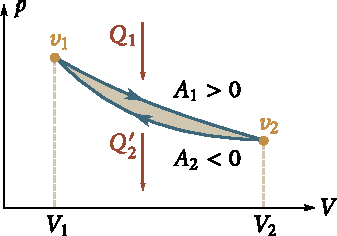
\includegraphics[scale=1.0]{figures/ch_12/fig_12_1.pdf}
		\caption[]{}
		\label{fig:12_1}
	\end{center}
	\vspace{-0.8cm}
\end{figure}

The working substance returns to its initial state upon completing a cycle. Therefore, the change in the internal energy during a cycle equals zero. The amount of heat supplied to the working substance during a cycle is $Q_1-Q_2'$, where $Q_1$ is the heat received by the working substance in expansion, and $Q_2'$ is the heat given up in compression. The work $A$ done during a cycle equals the area of the cycle (see Sec.~\ref{sec:10_6}). Equation~\eqref{eq:12_1} written for a cycle thus has the form
\begin{equation}\label{eq:12_3}
	A = Q_1 - Q_2'.
\end{equation}

A periodically functioning machine doing work at the expense of heat received from an external source is called a \textbf{heat engine}. We can see from \eqn{12_3} that not all the heat $Q_1$ received from an external source is used to obtain useful work. For a machine or engine to operate in cycles, part of the heat equal to $Q_1$ must be returned to the surroundings and is therefore not used for its direct purpose (\ie, for doing useful work). It is clear that the more completely a heat engine converts the heat $Q_1$ received from a source into useful work $A$, the more profitable is this engine. It is therefore customary practice to characterize a heat engine by its \textbf{efficiency} $\eta$ determined as the ratio of the work $A$ done during a cycle to the heat $Q_1$ received during the cycle:
\begin{equation}\label{eq:12_4}
	\eta = \frac{A}{Q_1}.
\end{equation}

\noindent
In view of \eqn{12_3}, the expression for the efficiency can be written in the form
\begin{equation}\label{eq:12_5}
	\eta = \frac{Q_1 - Q_2'}{Q_1}.
\end{equation}

\noindent
It follows from the definition of the efficiency that it cannot be greater than unity.

If we reverse the cycle shown in \fig{12_1}, we shall get a cycle of a refrigerating machine. Such a machine removes the heat $Q_2'$ from a substance at the temperature $T_2$ and gives up the heat $Q_1$ to a substance with a higher temperature $T_1$. The work $A'$ must be done on the machine during a cycle. The effectiveness of a refrigerating machine is characterized by its \textbf{refrigerating factor} (or \textbf{coefficient of performance}) $\beta$. The latter is defined as the ratio of the heat $Q_2$ removed from a body being cooled to the work $A'$ spent to actuate the machine:
\begin{equation}\label{eq:12_6}
	\beta = \frac{Q_2}{A'} = \frac{Q_2}{Q_1' - Q_2}.
\end{equation}

The second law of thermodynamics, like the first one, can be formulated in several ways. We have acquainted ourselves with one of them in Sec.~\ref{sec:11_11}. It is the statement that \textit{the entropy of an isolated system cannot diminish}:
\begin{equation}\label{eq:12_7}
	\deriv{S} \geqslant 0.
\end{equation}

The German physicist Rudolf Clausius (1822-1888) stated the second law as follows: \textit{processes are impossible whose only final result would be the flow of heat from a colder body to a warmer one}. Matters must not be understood in such a way that the second law in general prohibits the transfer of heat from a colder body to a warmer one. It is exactly such a transfer that is performed in a refrigerating machine. This transfer, however, is not the only result of a process. It is attended by changes in the surrounding bodies associated with the performance of the work $A'$ on the system.

We shall show that an imaginary process performed in an isolated system and contradicting the second law as worded by Clausius is attended by a decrease in the entropy. We shall thus prove the equivalence of Clausius's statement and of the statistical statement of the second law according to which the entropy of an isolated system cannot diminish.

We shall first make the following remark. Assume that a body exchanges heat with another body, which we shall call a \textbf{heat source} or \textbf{heat reservoir}. Let the heat capacity of the reservoir be infinitely great. This signifies that when the reservoir receives or gives up a finite amount of heat, its temperature does not change. A process occurring in a body and attended by the exchange of heat with a reservoir can be reversible only if in the course of this process the temperature of the body will equal that of the corresponding reservoir. Indeed, if, for example, a body receives heat from a reservoir having the temperature $T_1$  while having a temperature lower than $T_1$, then when the same process is reversed the body can return to the reservoir the heat received from it if its temperature at any rate is not lower than $T_1$. Consequently, in the forward and the reverse course of the process, the temperature of the body will differ, the body will pass in both cases through different sequences of states (characterized by different temperatures), and the process being considered will be irreversible.

Thus, a process attended by heat exchange can be reversible only if upon receiving heat and returning it in the reverse stroke to the reservoir, the body has the same temperature equal to that of the reservoir. Strictly speaking, when receiving heat, the temperature of the body must be lower than that of the reservoir by an infinitely small value (otherwise no heat will flow from the reservoir to the body), and when giving up heat, the temperature of the body must be higher than that of the reservoir by an infinitely small value.

Consequently, the only reversible process attended by heat exchange with a reservoir whose temperature remains constant is an isothermal process at the temperature of the reservoir. Let us consider an isolated system consisting of two bodies of the same heat capacity $C$. Assume that body B transfers the heat $Q$ to body A, and as a result the temperature of A rises from $\ab{T}{A,$0$}$ to $\ab{T}{A}$, while the temperature of B lowers from $\ab{T}{B,$0$}$ to $\ab{T}{B}$ (here $\ab{T}{B}<\ab{T}{B,$0$}<\ab{T}{A,$0$}<\ab{T}{A}$). Such a process contradicts the second law formulated by Clausius. Let us find the change in the entropy in this case. In the course of this process, heat exchange occurs between bodies with different temperatures. In view of what has been said above, such a process is irreversible. Equation~\eqref{eq:11_110}, however, may be applied only to reversible processes. To find the change in the entropy in an irreversible process, we proceed as follows. We consider a reversible process that brings the system to the same final state as the given irreversible process, and calculate the change in the entropy for this process by the equation
\begin{equation}\label{eq:12_8}
	S_2 - S_1 = \int_{1}^{2} \frac{\derivp{Q}}{T}
\end{equation}

\noindent
[see \eqn{11_110}].

In accordance with what has been said above, we shall consider a reversible process in the course of which body B gives up the heat $Q$ in portions of $\derivp{Q}$ to a consecutive series of reservoirs with temperatures having all the values from $\ab{T}{B,$0$}$ to $\ab{T}{B}$, and body A receives the heat $Q$ in portions of $\derivp{Q}$ from a number of reservoirs with temperatures from $\ab{T}{A,$0$}$ to $\ab{T}{A}$. As a result, the system will pass reversibly from the state in which the bodies have the temperatures $\ab{T}{A,$0$}$ and $\ab{T}{B,$0$}$ to the state in which the temperatures of the bodies are $\ab{T}{A}$ and $\ab{T}{B}$. The increment of the entropy in the course of this process is
\begin{align*}
	\Delta S &= \Delta\ab{S}{A} + \Delta\ab{S}{B} = \int_{\ab{T}{A,$0$}}^{\ab{T}{A}} \frac{C\,\deriv{T}}{T} + \int_{\ab{T}{B,$0$}}^{\ab{T}{B}} \frac{C\,\deriv{T}}{T}\\
	&= C\ln\parenthesis{\frac{\ab{T}{A}}{\ab{T}{A,$0$}}} + C\ln\parenthesis{\frac{\ab{T}{B}}{\ab{T}{B,$0$}}} = C\ln\parenthesis{\frac{\ab{T}{A}\ab{T}{B}}{\ab{T}{A,$0$}\ab{T}{B,$0$}}}.
\end{align*}

\noindent
Taking into account that $\ab{T}{A}=\ab{T}{A,$0$}+\alpha$ and $\ab{T}{B}=\ab{T}{B,$0$}-\alpha$ (here $\alpha=Q/C>0$), we can write $\Delta S$ in the form
\begin{equation*}
	\Delta S = C\ln\bracket{\frac{(\ab{T}{A,$0$}+\alpha)(\ab{T}{B,$0$}-\alpha)}{\ab{T}{A,$0$}\ab{T}{B,$0$}}} = C\ln\bracket{1 - \frac{\alpha (\ab{T}{A,$0$} - \ab{T}{B,$0$})}{\ab{T}{A,$0$}\ab{T}{B,$0$}} - \frac{\alpha^2}{\ab{T}{A,$0$}\ab{T}{B,$0$}}}.
\end{equation*}

\noindent
Since $\ab{T}{A,$0$}>\ab{T}{B,$0$}$, the expression in brackets is less than unity, and, consequently, $\Delta S<0$. We have thus shown that in the course of an imaginary process contradicting the second law as stated by Clausius, the entropy diminishes, which contradicts the law of non-diminishing of the entropy.

The British scientist Lord Kelvin (William Thomson, 1824-1907) proposed still another statement of the second law of thermodynamics. It is worded as follows: \textit{such processes are impossible whose only final result would be the removal of a definite amount of heat from a body and the complete conversion of this heat into work}.

It may seem on the face of it that this statement contradicts, for example, the process of isothermal expansion of an ideal gas. Indeed, all the heat received by an ideal gas from a body is completely converted into work. The reception of heat and its conversion into work are not the only final result of the process, however; as a result of the process the volume of the gas changes.

In a heat engine, the conversion of heat into work is attended without fail by an additional process---the transfer of a certain amount of heat $Q_2'$ to the colder body. Hence, the heat $Q_1$ received from the warmer body cannot be completely converted into work.

It is easy to see that Kelvin's statement logically follows from that of Clausius. Indeed, work can be completely transformed into heat, for example, in friction. Therefore, by using a process forbidden by Kelvin's statement to convert the heat removed from a body completely into work, and then transforming this work by friction into heat transferred to another body with a higher temperature, we would carry out a process that is impossible according to Clausius's statement.

By using processes forbidden by the second law of thermodynamics, we could create an engine doing work at the expense of the heat received from such a virtually inexhaustible source of energy, for example, as the ocean. In practice, such an engine would be equivalent to a perpetual motion machine. This is why the second law of thermodynamics is sometimes stated as follows: \textit{a perpetual motion machine of the second kind is impossible, \ie, such a periodically operating engine that would receive heat from a single reservoir and completely convert this heat into work}.

\section{The Carnot Cycle}\label{sec:12_2}

It can be seen from the preceding section that the presence of two heat reservoirs is needed for the operation of a heat engine. In the course of a cycle, the engine receives the heat $Q_1$ from one of them having the higher temperature $T_1$ and called the \textbf{high temperature reservoir} (or \textbf{heater}, or \textbf{heat source}). The engine gives up the heat $Q_2'$ to the second one having the lower temperature $T_2$ and called the \textbf{low temperature reservoir} (or \textbf{cooler}, or \textbf{heat sink}).

Let us assume that the heat capacity of the reservoirs is infinitely great. This signifies that when the reservoirs give up or receive a finite amount of heat, their temperatures do not change. Let us see what reversible cycle can be performed by the working substance of the engine in these conditions. For brevity's sake, we shall call the working substance of the engine simply the substance.

The cycle being considered can evidently consist both of processes during which the substance exchanges heat with the reservoirs, and of processes not attended by heat exchange with the surroundings, \ie, adiabatic processes. We established in the preceding section that the only reversible process attended by heat exchange with a reservoir whose temperature remains constant is an isothermal process going on at the temperature of the reservoir.

We thus arrive at the conclusion that a reversible cycle performed by a substance exchanging heat with two heat reservoirs of infinitely great capacity can consist only of two isotherms (at the temperatures of the reservoirs) and two adiabats. Such a cycle was first proposed for consideration by the French engineer Sadi Carnot (1796-1832) and is called the \textbf{Carnot cycle}. It must be noted that the Carnot cycle is reversible by definition.

In an adiabatic process, $\derivp{Q}=0$. Hence, according to \eqn{11_110}, in a reversible adiabatic process $\deriv{S}=0$ and, consequently, the entropy remains constant. This is why a reversible adiabatic process is called \textbf{isentropic}. Using this term, we can say that a Carnot cycle consists of two isotherms and two isentropes. In a $T$-$S$ diagram, this cycle appears as shown in \fig{12_2}. We must note that the shape of a Carnot cycle in a $T$-$S$ diagram does not depend on the properties of the substance (or system of substances) for which it is depicted.

\begin{figure}[t]
	\begin{minipage}[t]{0.5\linewidth}
		\begin{center}
			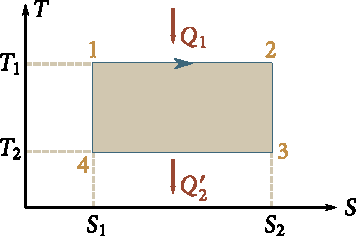
\includegraphics[scale=1.0]{figures/ch_12/fig_12_2.pdf}
			\caption[]{}
			\label{fig:12_2}
		\end{center}
	\end{minipage}
	\hspace{-0.05cm}
	\begin{minipage}[t]{0.5\linewidth}
		\begin{center}
			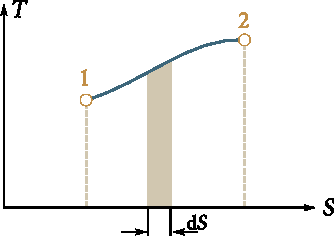
\includegraphics[scale=1.0]{figures/ch_12/fig_12_3.pdf}
			\caption[]{}
			\label{fig:12_3}
		\end{center}
	\end{minipage}
	\vspace{-0.4cm}
\end{figure}

Figure~\ref{fig:12_3} shows a process that transfers a system from state $1$ to state $2$. According to \eqn{11_110}, the elementary amount of heat $\derivp{Q}$ received by the system can be represented in the form $T\,\deriv{S}$. Hence, the area of the shaded strip in \fig{12_3} equals $\derivp{Q}$, and the area of the figure confined by curve $1$-$2$ gives the amount of heat received by the system in the course of the process. Similarly, the area of the figure confined by the curve depicting the process in a $p$-$V$ diagram gives the work done by the system in the course of the process (see \fig{10_4}).

In accordance with the above, the area of the cycle in \fig{12_2} gives the heat received by the system in the course of the cycle (it equals $Q_1-Q_2'$). Similarly, the area of the cycle in a $p$-$V$ diagram gives the work done by the system during the cycle (see \fig{10_5}).

The heat received by a system in the course of an arbitrary reversible process can be calculated by the formula
\begin{equation}\label{eq:12_9}
	Q = \int_{1}^{2} T\,\deriv{S}
\end{equation}

\noindent
[compare with \eqn{10_12}].

Let us find the efficiency of a Carnot cycle. Upon completing the cycle, the system returns to its initial state. Hence, the total change in the entropy during the cycle is zero. Along path $1$-$2$ (see \fig{12_2}), the system receives the heat $Q_1$ from the reservoir with the temperature $T_1$. The entropy increment on this path is
\begin{equation*}
	\Delta S_{12} = \int_{1}^{2} \frac{\derivp{Q}}{T_1} = \frac{1}{T_1} \int_{1}^{2} \derivp{Q} = \frac{Q_1}{T_1}.
\end{equation*}

\noindent
Along path $3$-$4$, the system gives up the heat $Q_2'$ to the reservoir with the temperature $T_2$. The removal of the heat $Q_2'$ from a substance is equivalent to supplying the heat $-Q_2'$ to it. Therefore, the entropy increment along path $3$-$4$ is
\begin{equation*}
	\Delta S_{34} = \int_{3}^{4} \frac{\derivp{Q}}{T_2} = \frac{1}{T_2} \int_{3}^{4} \derivp{Q} = -\frac{Q_2'}{T_2}.
\end{equation*}

\noindent
The entropy is constant along $2$-$3$ and $4$-$1$. Thus, the total entropy increment during the cycle is
\begin{equation}\label{eq:12_10}
	\Delta S_{12} + \Delta S_{34} = \frac{Q_1}{T_1} - \frac{Q_2'}{T_2} = 0.
\end{equation}

\noindent
It can be seen from \eqn{12_10} that
\begin{equation}\label{eq:12_11}
	\frac{Q_1}{T_1} = \frac{Q_2'}{T_2}.
\end{equation}

Equation~\eqref{eq:12_5} for the efficiency of a heat engine can be written in the form
\begin{equation}\label{eq:12_12}
	\eta = \frac{Q_1-Q_2'}{Q_1} = 1 - \frac{Q_2'}{Q_1}.
\end{equation}

\noindent
Substituting in this equation for $Q_2'/Q_1$ its value from \eqn{12_11}, we get
\begin{equation}\label{eq:12_13}
	\eta = 1 - \frac{T_2}{T_1} = \frac{T_1 - T_2}{T_1}.
\end{equation}

In deriving \eqn{12_13}, we made no assumptions on the properties of the working substance and the design of the heat engine. We thus arrive at the statement that \textit{the efficiency of all reversible machines operating in identical conditions (\ie, at the same temperatures of the hot temperature and cold temperature reservoirs) is the same and is determined only by the temperatures of the two reservoirs}. This statement is known as the \textbf{Carnot theorem}.

Let us consider an irreversible machine operating with the hot temperature and cold temperature reservoirs similar to those of a reversible machine operating according to the Carnot cycle. Assume that upon completion of the cycle the machine returns to its initial state, which we shall consider an equilibrium one. Since the entropy is a function of state, its increment during the cycle should equal zero:
\begin{equation*}
	\oint \deriv{S} = 0.
\end{equation*}

Since the processes which the cycle consists of are irreversible, for each elementary process the inequality $\deriv{S}>\derivp{Q}/T$ holds [see expression~\eqref{eq:11_111}). Hence, from the condition that the total entropy increment during the cycle equals zero, it follows that
\begin{equation*}
	0 = \oint \deriv{S} > \oint \frac{\derivp{Q}}{T}
\end{equation*}

\noindent
whence
\begin{equation}\label{eq:12_14}
	\oint \frac{\derivp{Q}}{T} < 0.
\end{equation}

\noindent
Let us divide the integral in~\eqref{eq:12_14} into four addends:
\begin{equation}\label{eq:12_15}
	\oint \frac{\derivp{Q}}{T} = \int_{T_1} \frac{\derivp{Q}}{T} + \int_{\text{Ad}1} \frac{\derivp{Q}}{T} + \int_{T_2} \frac{\derivp{Q}}{T} + \int_{\text{Ad}2} \frac{\derivp{Q}}{T} < 0.
\end{equation}

\noindent
The first addend corresponds to the process of obtaining the heat $Q_1$ (this amount of heat does not necessarily coincide with the heat $Q_1$ which a reversible machine receives during a cycle) from the reservoir with the temperature $T_1$. The second addend in~\eqref{eq:12_15} corresponds to the first adiabatic path of the cycle. The third addend corresponds to the process of transferring the heat $Q_2'$ (this amount of heat does not necessarily coincide with the heat $Q_2'$ which a reversible machine gives up during a cycle) to the reservoir with the temperature $T_2$. Finally, the fourth addend in~\eqref{eq:12_15} corresponds to the second adiabatic path of the cycle. On the adiabatic paths, $\derivp{Q}=0$, therefore the corresponding integrals vanish. The integral corresponding to the path $T_1$ equals $Q_1/T_1$ (we remind our reader that for an irreversible process, the denominator of the ratio $\derivp{Q}/T$ contains the temperature of the reservoir from which the given substance receives the heat $\derivp{Q}$). The integral corresponding to the path $T_2$ equals $-Q_2'/T_2$. We thus arrive at the inequality
\begin{equation}\label{eq:12_16}
	\frac{Q_1}{T_1} - \frac{Q_2'}{T_2}  < 0.
\end{equation}

\noindent
We find from~\eqref{eq:12_16} that
\begin{equation*}
	\frac{Q_2'}{Q_1} > \frac{T_2}{T_1}
\end{equation*}

\noindent
and, consequently,
\begin{equation}\label{eq:12_17}
	\eta = 1 - \frac{Q_2'}{Q_1} < 1 - \frac{T_2}{T_1} = \frac{T_1 - T_2}{T_1}.
\end{equation}

\noindent
The result obtained signifies that the efficiency of an irreversible machine is always smaller than that of a reversible one operating in the same conditions.

\begin{figure}[t]
	\begin{center}
		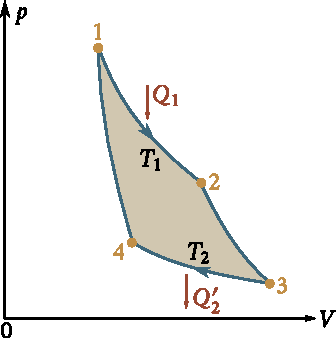
\includegraphics[scale=1.0]{figures/ch_12/fig_12_4.pdf}
		\caption[]{}
		\label{fig:12_4}
	\end{center}
	\vspace{-0.8cm}
\end{figure}

The form of a Carnot cycle in a $p$-$V$ diagram depends on the properties of the substance performing the cycle. A cycle for an ideal gas is shown in \fig{12_4}. The efficiency of a Carnot cycle for an ideal gas can be calculated without resorting to finding the entropy increment.

The internal energy of an ideal gas remains constant in an isothermal process. Therefore, the heat $Q_1$ received by the gas equals the work $A_{12}$ done by the gas upon transition from state $1$ to state $2$ (\fig{12_4}). This work, according to \eqn{10_60}, is
\begin{equation}\label{eq:12_18}
	Q_1 = A_{12} = \frac{m}{M}RT_1 \ln\parenthesis{\frac{V_2}{V_1}}
\end{equation}

\noindent
where $m$ is the mass of the ideal gas in the machine. The heat $Q_2'$ given up to the low temperature reservoir equals the work $A_{34}'$ done to compress the gas from state $3$ to state $4$. This work is
\begin{equation}\label{eq:12_19}
	Q_2' = A_{34}' = \frac{m}{M}RT_2 \ln\parenthesis{\frac{V_3}{V_4}}.
\end{equation}

For the cycle to be closed, states $1$ and $4$ must be on the same adiabat. Hence the condition follows that
\begin{equation}\label{eq:12_20}
	T_1 V_1^{\gamma-1} = T_2 V_2^{\gamma-1}.
\end{equation}

\noindent
[see adiabat equation~\eqref{eq:10_41}]. Similarly, since states $2$ and $3$ are on the same adiabat, the condition is observed that
\begin{equation}\label{eq:12_21}
	T_3 V_3^{\gamma-1} = T_4 V_4^{\gamma-1}.
\end{equation}

\noindent
By dividing \eqn{12_21} by~\eqref{eq:12_20}, we arrive at the condition for the cycle to be closed:
\vspace{-12pt}
\begin{equation}\label{eq:12_22}
	\frac{V_2}{V_1} = \frac{V_3}{V_4}.
\end{equation}

Now let us introduce Eqs.~\eqref{eq:12_18} and~\eqref{eq:12_19} into \eqn{12_5} for the efficiency:
\begin{equation*}
	\eta = \frac{\dfrac{m}{M}RT_1\ln\parenthesis{\dfrac{V_2}{V_1}} - \dfrac{m}{M}RT_2\ln\parenthesis{\dfrac{V_3}{V_4}}}{\dfrac{m}{M}RT_1\ln\parenthesis{\dfrac{V_2}{V_1}}}.
\end{equation*}

\noindent
Finally, taking condition~\eqref{eq:12_22} into account, we get
\begin{equation*}
	\eta = \frac{T_1 - T_2}{T_1}
\end{equation*}

\noindent
which coincides with \eqn{12_13}.

\section{The Thermodynamic Temperature Scale}\label{sec:12_3}

The theorem on the efficiency of reversible machines not depending on the properties of the working substance proved in the preceding section makes it possible to establish a temperature scale that does not depend on the choice of the thermometric body. In accordance with this theorem, the quantity
\begin{equation*}
	\eta = \frac{Q_1 - Q_2'}{Q_1} = 1 - \frac{Q_2'}{Q_1}
\end{equation*}

\noindent
and, consequently, the ratio $Q_2'/Q_1$ for a Carnot cycle depend only on the temperature of the high temperature and low temperature reservoirs. Denoting the values of these temperatures according to a scale that we meanwhile do not know by $\theta_1$ and $\theta_2$, we can write that
\begin{equation}\label{eq:12_23}
	\frac{Q_2'}{Q_1} = f(\theta_1,\theta_2)
\end{equation}

\noindent
where $f(\theta_1,\theta_2)$ is a universal (\ie, identical for all Carnot cycles) function of the high temperature and low temperature reservoirs. Equation~\eqref{eq:12_23} permits us to determine the temperature of bodies through the amounts of heat received and given up in Carnot cycles.

We shall prove that function~\eqref{eq:12_23} has the following property:
\begin{equation}\label{eq:12_24}
	f(\theta_1,\theta_2) = \frac{\Theta(\theta_2)}{\Theta(\theta_1)}
\end{equation}

\noindent
where $\Theta(\theta)$ is again a universal function of the temperature. Let us consider two reversible machines M$_1$ and M$_2$ (\fig{12_5}), the cooler (low temperature reservoir) of one of them simultaneously being the heater (high temperature reservoir) of the other. Let the second machine take the same amount of heat from the reservoir at the temperature $\theta_1$ that the first machine supplies to it.

\begin{figure}[t]
	\begin{center}
		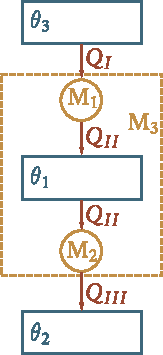
\includegraphics[scale=1.0]{figures/ch_12/fig_12_5.pdf}
		\caption[]{}
		\label{fig:12_5}
	\end{center}
	\vspace{-0.8cm}
\end{figure}

For machine M$_1$ , we have $Q_1=Q_I$ and $Q_2'=Q_{II}$. Hence, \eqn{12_23} for this machine has the form
\begin{equation}\label{eq:12_25}
	\frac{Q_{II}}{Q_I} = f(\theta_3,\theta_1).
\end{equation}

\noindent
For machine M$_2$, we have $Q_1=Q_{II}$, $Q_2'=Q_{III}$. Hence, by \eqn{12_23},
\begin{equation}\label{eq:12_26}
	\frac{Q_{III}}{Q_{II}} = f(\theta_1,\theta_2).
\end{equation}

\noindent
Considering machines M$_1$ and M$_2$, and also the reservoir with the temperature $\theta_1$ as a single reversible machine that receives the heat $Q_I$ from the heater with the temperature $\theta_3$ and gives up the heat $Q_{III}$ to the cooler with the temperature $\theta_2$, we can write:
\begin{equation}\label{eq:12_27}
	\frac{Q_{III}}{Q_{I}} = f(\theta_3,\theta_2).
\end{equation}

Dividing \eqn{12_27} by~\eqref{eq:12_25}, we find that
\begin{equation*}
	\frac{Q_{III}}{Q_{II}} = \frac{f(\theta_3,\theta_2)}{f(\theta_3,\theta_1)}.
\end{equation*}

\noindent
A comparison of this equation with \eqn{12_26} gives us the expression
\begin{equation}\label{eq:12_28}
	f(\theta_1,\theta_2) = \frac{f(\theta_3,\theta_2)}{f(\theta_3,\theta_1)}.
\end{equation}

\noindent
This equation relates the temperatures $\theta_1$ and $\theta_2$ of two substances, but the temperature $\theta_3$ of a third substance figures in it. If we agree once and forever on the selection of this substance, \ie, make $\theta_3$ constant, we shall reduce the function $f(\theta_3,\theta)$ in the numerator and denominator of \eqn{12_28} to a function of a single variable $\theta$. Denoting this function by $\Theta(\theta)$ we arrive at \eqn{12_24}.

The function $\Theta(\theta)$ depends only on the temperature. Therefore its value can be used to characterize the temperature of the corresponding substance, \ie, assume that the temperature of the substance is $\Theta$, where $\Theta=\Theta(\theta)$. Equation~\eqref{eq:12_23} thus becomes
\begin{equation}\label{eq:12_29}
	\frac{Q_2'}{Q_1} = \frac{\Theta_2}{\Theta_1}.
\end{equation}

\noindent
Equation~\eqref{eq:12_29} is the foundation of the so-called \textbf{thermodynamic temperature scale}. A merit of this scale is that it does not depend on the choice of the substance (the working substance in a Carnot cycle) used for measuring the temperature.

In accordance with \eqn{12_29}, to compare the temperatures of two bodies, we must carry out a Carnot cycle using these bodies as the high temperature and low temperature reservoirs. The ratio of the amount of heat given up to the ``low temperature reservoir'' body to the amount of heat removed from the ``high temperature reservoir'' body gives the ratio of the temperatures of the two bodies. To uniquely determine the numerical value of $\Theta$, we must come to an agreement on the choice of the temperature unit, \ie, the degree. The absolute degree is defined as one-hundredth of the difference between the temperature of water boiling at atmospheric pressure and that of melting ice. Thus, the degree of the absolute thermodynamic scale equals the degree of the ideal gas scale.

It is easy to see that the thermodynamic temperature scale coincides with the ideal gas scale. Indeed, according to \eqn{12_11}, we have
\begin{equation}\label{eq:12_30}
	\frac{Q_2'}{Q_1} = \frac{T_2}{T_1}.
\end{equation}

\noindent
Comparing Eqs.~\eqref{eq:12_29} and~\eqref{eq:12_30}, we find that
\begin{equation*}
	\frac{\Theta_2}{\Theta_1} = \frac{T_2}{T_1}.
\end{equation*}

\noindent
Hence, $\Theta$ is proportional to $T$, and since the degree of both scales is the same, $\Theta=T$.

\section{Examples of Calculating the Entropy}\label{sec:12_4}

The entropy is a function of state. It must therefore depend on parameters determining the state of a system. For example, it can be represented as a function of $p$ and $T$, or as a function of $V$ and $T$, and so on. Let us assume that a body is heated at the constant pressure $p$ from absolute zero to the temperature $T$, and that the heating process is reversible. Hence, according to Eqs.~\eqref{eq:11_110} and~\eqref{eq:10_24}, the entropy of a body at the pressure $p$ and temperature $T$ is determined by the expression
\begin{equation}\label{eq:12_31}
	S(p,T) = \int_{0}^{T} \frac{C_p(T)\,\deriv{T}}{T}
\end{equation}

\noindent
where $C_p(T)$ is the heat capacity of the body at constant pressure, which is a function of temperature. Similarly, the entropy as a function of the volume $V$ and temperature $T$ can be represented in the form
\begin{equation}\label{eq:12_32}
	S(V,T) = \int_{0}^{T} \frac{C_V(T)\,\deriv{T}}{T}
\end{equation}

\noindent
where $C_V$ is the heat capacity of the body at constant volume.

It can be seen from Eqs.~\eqref{eq:12_31} and~\eqref{eq:12_32} that the heat capacities $C_p$ and $C_V$ (and also the heat capacity in any other process) vanish at absolute zero. Indeed, if the heat capacity did not tend to zero, then the integrand at $T$ tending to zero would grow without restriction, as a result of which the integral would be diverging (\ie, would become infinite).

\textbf{1. Entropy of an Ideal Gas}. In Sec.~\ref{sec:11_11}, we found an expression for the entropy of a monatomic ideal gas (\ie, a gas for which $C_V=3R/2$). Now, using \eqn{11_110}, we shall get an expression for the entropy of an ideal gas with any molecules. Since the entropy is additive, it is sufficient to find its value for a mole of the gas $\ab{S}{m}$. The entropy of an arbitrary amount of the gas will be $S=(m/M)\ab{S}{m}$.

We shall characterize the state of a substance by the parameters $V$ and $T$, but shall not consider that the process being studied is isochoric. According to Nernst's theorem and \eqn{11_110}, we have
\begin{equation}\label{eq:12_33}
	\ab{S}{m}(V,T) = \int_{0}^{(V,T)} \frac{\derivp{Q}}{T}
\end{equation}

\noindent
where the symbol $(V, T)$ designates the state of the gas (we have in mind the volume of a mole). Integration is performed over an arbitrary reversible process transferring the substance from its state at absolute zero to the state characterized by the volume $V$ and the temperature $T$.

Let us take the volume $V_0$ and the temperature $T_0$ at which the substance is sure to be an ideal gas, and divide the integral in \eqn{12_33} into two:
\begin{equation}\label{eq:12_34}
	\ab{S}{m}(V,T) = \int_{0}^{(V_0,T_0)} \frac{\derivp{Q}}{T} + \int_{(V_0,T_0)}^{(V,T)} \frac{\derivp{Q}}{T}.
\end{equation}

\noindent
The first integral is a number that we shall denote by $S(V_0,T_0)$. The second integral is a function of $V$ and $T$. To find the form of this function, let us write $\derivp{Q}$ as $\derivp{Q}=C_V\,\deriv{T}+p\,\deriv{V}$ (in the integration interval the substance behaves like an ideal gas). Dividing $\derivp{Q}$ by $T$ and substituting $R/V$ for $p/T$ in accordance with an equation of state, we get
\begin{equation*}
	\int_{(V_0,T_0)}^{(V,T)} \frac{\derivp{Q}}{T} = \int_{T_0}^{T} \frac{C_V\,\deriv{T}}{T} + \int_{V_0}^{V} \frac{R\,\deriv{V}}{V} = C_V\ln\parenthesis{\frac{T}{T_0}} + R\ln\parenthesis{\frac{V}{V_0}}.
\end{equation*}

\noindent
Thus, \eqn{12_34} becomes
\begin{equation}\label{eq:12_35}
	\ab{S}{m}(V,T) = S(V_0,T_0) + C_V\ln\parenthesis{\frac{T}{T_0}} + R\ln\parenthesis{\frac{V}{V_0}}.
\end{equation}

\noindent
We can transform this equation as follows\footnote{One must not be confused in seeing a quantity having a dimension inside a logarithm. Expressions containing $\ln{f}$ always have an addend including $\ln{f_0}$ ($f_0$ is a constant) with a sign such that $\ln{f}$ and $\ln{f_0}$ can be combined into a single addend of the kind $\ln(f/f_0)$.}
\begin{equation}\label{eq:12_36}
	\ab{S}{m} = C_V\ln{T} + R\ln{V} + S_0
\end{equation}

\noindent
where $S_0$ is a constant equal to $S(V_0,T_0)-\ln{T_0}-\ln{V_0}$.

It must be noted that the relations with which we have to deal in practice usually include either derivatives of the entropy with respect to parameters of state or a change in the entropy. In these cases, there is no need to find the value of the additive constant in the expression for the entropy.

Equation~\eqref{eq:12_36} gives an expression for the entropy of a mole of an ideal gas in variable $V$ and $T$. We can use an equation of state to pass over to expressions for the entropy in other variables. Using $V=RT/p$ in \eqn{12_36}, we get
\begin{equation*}
	\ab{S}{m} = C_V\ln{T} + R\ln{R} + R\ln{T} - R\ln{p} + S_0.
\end{equation*}

\noindent
Taking into account that for an ideal gas $C_V+R=C_p$, we can
write
\begin{equation}\label{eq:12_37}
	\ab{S}{m} = C_p\ln{T} + R\ln{p} + S_0'
\end{equation}

\noindent
where $S_0'=S_0+R\ln{R}$.

Finally, substituting $pV/R$ for $T$ in \eqn{12_36}, we arrive at the equation
\begin{equation}\label{eq:12_38}
	\ab{S}{m} = C_V\ln{p} + C_p\ln{V} + S_0''
\end{equation}

\noindent
where $S_0''=S_0-V_C\ln{R}$.

\textbf{2. Entropy of Water.} The changes in the heat capacity of water within the interval from \SIrange{0}{100}{\degreeCelsius} do not exceed 1\%. Therefore, 	within this temperature interval, the specific heat capacity of water may be considered constant and equal to $c=\SI{4.2}{\kilo\joule\per\kilo\gram\per\kelvin}$. Accordingly, denoting by $s(273)$ the specific entropy of liquid water at \SI{0}{\degreeCelsius} and by $s(T)$ the specific entropy of water at the temperature $T$ (here $273<T<373$), we can write that
\begin{equation*}
	s(T) - s(273) \int_{273}^{T} \frac{c\,\deriv{T}}{T} = c\ln\parenthesis{\frac{T}{273}}
\end{equation*}

\noindent
whence
\begin{equation}\label{eq:12_39}
	s(T) = c\ln{T} + [s(273) - c\ln(273)] = c\ln{T} + \text{constant}.
\end{equation}

\textbf{3. Change in Entropy in Melting.} If the pressure does not change, then melting proceeds at a constant temperature. Accordingly, the increment of the specific entropy is
\begin{equation}\label{eq:12_40}
	\Delta s = \int_{\text{sol}}^{\text{liq}} \frac{\derivp{Q}}{\ab{T}{f}} = \frac{1}{\ab{T}{f}} \int_{\text{sol}}^{\text{liq}} \derivp{Q} = \frac{\ab{L}{f}}{\ab{T}{f}}
\end{equation}

\noindent
where $\ab{L}{f}$ is the specific heat of fusion. When a substance solidifies, its specific entropy diminishes by the same amount.

The formula for the increment of the specific entropy upon evaporation differs from \eqn{12_40} only in that it includes the heat of vaporization and the boiling point instead of the heat of fusion and the melting point.

\section{Some Applications of Entropy}\label{sec:12_5}

Let us take the volume $V$ and the temperature $T$ as the independent parameters characterizing the state of a substance. Hence, the internal energy of the substance will be a function of these parameters: $U=U(V, T)$. In this case, the expression of the first law of thermodynamics has the form\footnote{The total differential of the function $f(x,y)$ of the variables $x$ and $y$ is determined by the expression $\deriv{f}=\diffinpartial{f}{x}\,\deriv{x}+\diffinpartial{f}{y}\,\deriv{y}$. This expression gives the increment of the function $f(x,y)$ when the variables $x$ and $y$ receive the increments $\deriv{x}$ and $\deriv{y}$ [see \eqn{3_33}].}
\begin{equation}\label{eq:12_41}
	\derivp{Q} = \parenthesis{\diffpartial{U}{T}}_V\,\deriv{T} + \parenthesis{\diffpartial{U}{V}}_T\,\deriv{V} + p\,\deriv{V}.
\end{equation}

\noindent
It is customary practice in thermodynamics to write partial derivatives of functions with respect to the state parameters with a subscript indicating what parameter is assumed to be constant in differentiation. This is essential in connection with the fact that, for example, we can consider the partial derivative of $U$ with respect to $T$ provided that $p$ remains constant. This derivative is denoted by the symbol $(\diffinpartial{U}{T})_p$ and, generally speaking, has a different value than $(\diffinpartial{U}{T})_V$.

Dividing \eqn{12_41} by $T$, we get the increment of the entropy:
\begin{equation}\label{eq:12_42}
	\deriv{S} = \bracket{\frac{1}{T} \parenthesis{\diffpartial{U}{T}}_V} \, \deriv{T} + \bracet{\frac{1}{T} \bracket{\parenthesis{\diffpartial{U}{V}}_T + p}}\,\deriv{V}.
\end{equation}

\noindent
Considering the entropy as a function of the parameters $V$ and $T$, we can write the increment of the entropy in the form
\begin{equation*}
	\deriv{S} = \parenthesis{\diffpartial{S}{T}}_V\,\deriv{T} + \parenthesis{\diffpartial{S}{V}}_T\,\deriv{V}.
\end{equation*}

\noindent
A comparison with \eqn{12_42} shows that
\begin{equation}\label{eq:12_43}
	\parenthesis{\diffpartial{S}{T}}_V = \frac{1}{T} \parenthesis{\diffpartial{U}{T}}_V,\quad \parenthesis{\diffpartial{S}{V}}_T = \frac{1}{T} \bracket{\parenthesis{\diffpartial{U}{V}}_T + p}.
\end{equation}

The mixed partial derivatives of a function $f(x, y)$ satisfy the condition
\begin{equation*}
	\frac{\uppartial^2f}{\uppartial x\,\uppartial y} = \frac{\uppartial^2f}{\uppartial y\,\uppartial x}.
\end{equation*}

\noindent
Accordingly,
\begin{equation*}
	\frac{\uppartial}{\uppartial V} \parenthesis{\diffpartial{S}{T}}_V = \frac{\uppartial}{\uppartial T} \parenthesis{\diffpartial{S}{V}}_T.
\end{equation*}

\noindent
The introduction of Eqs.~\eqref{eq:12_43} into this equation yields
\begin{equation*}
	\frac{\uppartial}{\uppartial V} \bracket{\frac{1}{T} \parenthesis{\diffpartial{U}{T}}_V} = \frac{\uppartial}{\uppartial T} \bracet{\frac{1}{T} \bracket{\parenthesis{\diffpartial{U}{V}}_T + p}}.
\end{equation*}

\noindent
After differentiation, we get
\begin{equation*}
	\frac{1}{T}\frac{\uppartial^2U}{\uppartial V\,\uppartial T} = -\frac{1}{T^2} \bracket{\parenthesis{\diffpartial{U}{V}}_T + p} + \frac{1}{T} \bracket{\frac{\uppartial^2U}{\uppartial T\,\uppartial V} + \parenthesis{\diffpartial{p}{T}}_V}.
\end{equation*}

\noindent
Taking into account that $\uppartial^2U/\uppartial V\,\uppartial T$, we arrive at the formula
\begin{equation}\label{eq:12_44}
	\parenthesis{\diffpartial{U}{V}}_T = T \parenthesis{\diffpartial{p}{T}}_V - p.
\end{equation}

The latter shows how the internal energy depends on the volume. Let us use it to find the internal energy of an ideal and a van der Waals gas.

For an ideal gas, we have $p=RT/V$. Hence, $(\diffinpartial{p}{T})_V=R/V$. Using this value in \eqn{12_44}, we obtain
\begin{equation*}
	\parenthesis{\diffpartial{U}{V}}_T = T\frac{R}{V} - p = 0.
\end{equation*}

\noindent
The result obtained signifies that the internal energy of an ideal gas does not depend on its volume. In Sec.~\ref{sec:10_9}, we arrived at the same conclusion when we assumed that there is no interaction between molecules.

It follows from the equation of state for a van der Waals gas [see \eqn{10_62}] that
\vspace{-12pt}
\begin{equation}\label{eq:12_45}
	p = \frac{RT}{(V - b)} - \frac{a}{V^2}.
\end{equation}

\noindent
Hence
\begin{equation*}
	\parenthesis{\diffpartial{p}{T}}_V = \frac{R}{(V-b)}.
\end{equation*}

\noindent
Using this expression in formula~\eqref{eq:12_44}, we get
\begin{equation*}
	\parenthesis{\diffpartial{U}{V}}_T = \frac{RT}{(V - b)} - p = \frac{a}{V^2}.
\end{equation*}

\noindent
[see \eqn{12_45}]. Integration with respect to $V$ yields
\begin{equation*}
	U = -\frac{a}{V} + f(T).
\end{equation*}

\noindent
The function $f(T)$ can be concreted by taking advantage of the fact that at $V$ tending to infinity the expression for the internal energy of a van der Waals gas must transform into the expression for the internal energy of an ideal gas $U=C_VT$. As a result, we arrive at the expression $U=C_VT-a/V$ which we obtained in Sec.~\ref{sec:10_13} on the basis of other considerations [see \eqn{10_66}].

\section{Thermodynamic Potentials}\label{sec:12_6}

All calculations in thermodynamics are based on the use of functions of state called \textbf{thermodynamic potentials}. A separate thermodynamic potential corresponds to each set of independent parameters. The changes in the potentials occurring in the course of processes determine either the work done by the system or the heat received by it.

In considering thermodynamic potentials, we shall use expression~\eqref{eq:11_112}, writing it in the form
\begin{equation}\label{eq:12_46}
	T\,\deriv{S} \geqslant \derivp{Q}.
\end{equation}

\noindent
The equality sign relates to reversible processes, the inequality sign to irreversible ones.

The thermodynamic potentials are functions of state. Therefore, the increment of any of the potentials equals the total differential of the function by which it is expressed. The total differential of the function $f(x, y)$ of the variables $x$ and $y$ is determined by the expression
\begin{equation*}
	\deriv{f} = \diffpartial{f}{x}\,\deriv{x} + \diffpartial{f}{y}\,\deriv{y}.
\end{equation*}

\noindent
Therefore, if in the course of transformations we get for the increment of a quantity fan expression of the kind
\begin{equation}\label{eq:12_47}
	\deriv{f} = X(\zeta,\eta)\,\deriv{\zeta} + Y(\zeta,\eta)\,\deriv{\eta}
\end{equation}

\noindent
then we can state that this quantity is a function of the parameters $\zeta$ and $\eta$), the functions $X(\zeta,\eta)$ and $Y(\zeta,\eta)$ being the partial derivatives of the function $f(\zeta,\eta)$:
\begin{equation}\label{eq:12_48}
	\parenthesis{\diffpartial{f}{\zeta}}_{\eta} = X(\zeta,\eta),\quad \parenthesis{\diffpartial{f}{\eta}}_{\zeta} = Y(\zeta,\eta).
\end{equation}

\textbf{Internal Energy.} We are already well acquainted with one of the thermodynamic potentials, namely, the internal energy of a system. The expression of the first law for a reversible process can be written in the form
\begin{equation}\label{eq:12_49}
	\deriv{U} = T\,\deriv{S} - p\,\deriv{V}.
\end{equation}

\noindent
A comparison with \eqn{12_47} shows that the variables $S$ and $V$ fill the capacity of the so-called natural variables for the potential $U$. It follows from \eqn{12_48} that
\begin{equation}\label{eq:12_50}
	\parenthesis{\diffpartial{U}{S}}_V = T,\quad 	\parenthesis{\diffpartial{U}{V}}_S = -p.
\end{equation}

It can be seen from the relation $\derivp{Q}=\deriv{U}+\derivp{A}$ that when a body does not exchange heat with surroundings, the work done by it is
\begin{equation*}
	\derivp{A} = -\deriv{U}
\end{equation*}

\noindent
or in the integral form
\begin{equation}\label{eq:12_51}
	A = U_1 - U_2. \quad \text{(heat exchange is absent)}
\end{equation}

\noindent
Thus, in the absence of heat exchange with the surroundings, the work equals the decrement of the internal energy of a body. At constant volume
\begin{equation}\label{eq:12_52}
	\derivp{Q} = \deriv{U}.
\end{equation}

\noindent
Hence, the heat capacity at constant volume is
\begin{equation}\label{eq:12_53}
	C_V = \parenthesis{\diffpartial{U}{T}}_V.
\end{equation}

\textbf{Free Energy.} According to \eqn{12_49}, the work done by a body in a reversible isothermal process can be written in the form
\begin{equation}\label{eq:12_54}
	\derivp{A} = - \deriv{U} + T\,\deriv{S} = -\deriv{(U - TS)}.
\end{equation}

\noindent
The function of state
\begin{equation}\label{eq:12_55}
	F = U - TS
\end{equation}

\noindent
is called the \textbf{free (Helmholtz) energy} of a body.

According to Eqs.~\eqref{eq:12_54} and~\eqref{eq:12_55}, in a reversible isothermal process, the work equals the decrement of the free energy of a body:
\begin{equation}\label{eq:12_56}
	\derivp{A} = -\deriv{F}
\end{equation}

\noindent
or
\begin{equation}\label{eq:12_57}
	A = F_1 - F_2.\quad \text{($T = $ constant, reversible)}
\end{equation}

\noindent
A comparison with \eqn{12_51} shows that in isothermal processes the free energy plays the same part as the internal energy in adiabatic ones.

We must note that \eqn{12_51} holds for both reversible and irreversible processes. Equation~\eqref{eq:12_57}, on the contrary, holds only for reversible processes. For irreversible processes, we have $\derivp{Q}<T\,\deriv{S}$ [see expression~\eqref{eq:12_46}]. Introducing this inequality into the equation $\derivp{A}=\derivp{Q}-\deriv{U}$, it is easy to find that in irreversible isothermal processes we have
\begin{equation}\label{eq:12_58}
	A < F_1 - F_2.\quad \text{($T = $ constant, irreversible)}
\end{equation}

\noindent
Hence, the decrement of the free energy determines the upper limit of the amount of work that a system can do in an isothermal process.

Let us take a differential of the function~\eqref{eq:12_55}. Taking \eqn{12_49} into account, we get
\begin{equation}\label{eq:12_59}
	\deriv{F} = T\,\deriv{S} -  p\,\deriv{V} - T\,\deriv{S} - S\,\deriv{T} = -S\,\deriv{T} - p\,\deriv{V}.
\end{equation}

\noindent
We conclude from a comparison with \eqn{12_47} that $T$ and $V$ are the natural variables for the free energy. According to \eqn{12_48}
\begin{equation}\label{eq:12_60}
	\parenthesis{\diffpartial{F}{T}}_V = -S,\quad \parenthesis{\diffpartial{F}{V}}_T = -p.
\end{equation}

Let us substitute $\deriv{U}+p\,\deriv{V}$ for $\derivp{Q}$ in expression~\eqref{eq:12_46} and divide the resulting relation by $\deriv{t}$ (here $t$ is the time). The result is
\begin{equation}\label{eq:12_61}
	T\,\diff{S}{t} \geqslant \diff{U}{t} + p\,\diff{V}{t}.
\end{equation}

\noindent
If the temperature and the volume remain constant, then expression~\eqref{eq:12_46} can be transformed as follows:
\vspace{2pt}
\begin{equation}\label{eq:12_62}
	\diff{(U-TS)}{t} = \diff{F}{t} \leqslant 0.\quad \text{($T = $ constant, $V = $ constant)}
\end{equation}

\noindent
Examination of this expression shows that an irreversible process occurring at constant temperature and volume is attended by a decrease in the free energy of the body. When equilibrium is reached, $F$ stops changing with time. Thus, a state for which the free energy is minimum is the equilibrium one at constant temperature and volume.

\textbf{Enthalpy.} If a process goes on at constant pressure, then the amount of heat received by a body can be represented as follows:
\begin{equation}\label{eq:12_63}
	\derivp{Q} = \deriv{U} + p\,\deriv{V} = \deriv{(U + pV)}.
\end{equation}

\noindent
The function of state
\begin{equation}\label{eq:12_64}
	H = U + pV
\end{equation}

\noindent
is called the \textbf{enthalpy} (or \textbf{heat function}).

It follows from Eqs.~\eqref{eq:12_63} and~\eqref{eq:12_64} that the heat received by a body in the course of an isobaric process is
\begin{equation}\label{eq:12_65}
	\derivp{Q} = \deriv{H}
\end{equation}

\noindent
or in the integral form
\begin{equation}\label{eq:12_66}
	Q = H_2 - H_1.
\end{equation}

\noindent
Hence, when the pressure remains constant, the heat received by a body equals the increment of the enthalpy.

Differentiation of \eqn{12_64} with account taken of \eqn{12_49} yields
\begin{equation}\label{eq:12_67}
	\deriv{H} = T\,\deriv{S} - p\,\deriv{V} + p\,\deriv{V} + V\,\deriv{p} = T\,\deriv{S} + V\,\deriv{p}.
\end{equation}

\noindent
Thus, we conclude that the enthalpy is a thermodynamic potential in the variables $S$ and $p$. Its partial derivatives are
\begin{equation}\label{eq:12_68}
	\parenthesis{\diffpartial{H}{S}}_p = T,\quad 	\parenthesis{\diffpartial{H}{p}}_S = V.
\end{equation}

The heat capacity at constant pressure in accordance with \eqn{12_65} is
\begin{equation}\label{eq:12_69}
	C_p = \parenthesis{\diffpartial{H}{T}}_p.
\end{equation}

\noindent
Comparing Eqs.~\eqref{eq:12_65} and~\eqref{eq:12_69} with~\eqref{eq:12_52} and~\eqref{eq:12_53}, we arrive at the conclusion that when the pressure is constant, the enthalpy has properties similar to those which the internal energy has at a constant volume.

\textbf{Gibbs Thermodynamic Potential.} This function of state (also called the \textbf{Gibbs energy)} is determined as follows:
\begin{equation}\label{eq:12_70}
	G = H - TS = U + pV - TS.
\end{equation}

\noindent
Its total differential is [see \eqn{12_67}]
\begin{equation}\label{eq:12_71}
	\deriv{G} = T\,\deriv{S} + V\,\deriv{p} - S\,\deriv{T} = V\,\deriv{p} - S\,\deriv{T}.
\end{equation}

\noindent
Consequently, $p$ and $T$ are the natural variables for the function $G$. The partial derivatives of this function are
\begin{equation}\label{eq:12_72}
	\parenthesis{\diffpartial{G}{p}}_T = V,\quad 	\parenthesis{\diffpartial{G}{T}}_p = -S.
\end{equation}

If the temperature and pressure remain constant, \eqn{12_61} can be written in the form
\begin{equation}\label{eq:12_73}
	\diff{(U+pV-TS)}{t} = \diff{G}{t} \leqslant 0.\quad \text{($T = $ constant, $p = $ constant)}
\end{equation}

\noindent
It can be seen from this expression that an irreversible process going on at constant temperature and pressure is attended by a decrease in the Gibbs thermodynamic potential. When equilibrium is reached, $G$ stops changing with time. Thus, a state for which the Gibbs thermodynamic potential is minimum is the equilibrium one at constant temperature and pressure [compare with expression~\eqref{eq:12_62}].

Table~\ref{table:12_1} gives the basic properties of the thermodynamic potentials.

\begin{table}[!b]
	\renewcommand{\arraystretch}{1.2}
	\caption{ }
	\vspace{-0.6cm}
	\label{table:12_1}
	\begin{center}\resizebox{0.98\linewidth}{!}{
			\begin{tabular}{p{0.39\linewidth} p{0.18\linewidth} p{0.41\linewidth}}
				\toprule[1pt]
				\textbf{Name and symbol of} &\\
				\textbf{thermodynamic potential}& \multicolumn{2}{c}{\textbf{Properties}}\\
				\midrule[0.5pt]\midrule[0.5pt]
				Internal energy & $U_1 - U_2 = A$ & in adiabatic process\\
				$\quad U=U(S,V)$ & $U_2 - U_1 = Q$ & when $V$ is constant\\
				\midrule[0.5pt]
				Free energy & $F_1 - F_2 = A$ & in irreversible isothermal process\\
				$\quad F=F(T,V)$ & $F=\text{min}$ & for equilibrium state when $T$ and $V$ are constants\\
				\midrule[0.5pt]
				Enhalpy & $H_2 - H_1 = Q$ & when $p$ is constant\\
				$\quad H = H(S,p)$ & & \\
				\midrule[0.5pt]
				Gibbs thermodynamic potential & $G=\text{min}$ & for equilibrium state when\\
				$\quad G=G(p,T)$ & & $T$ and $p$ are constants\\
				\bottomrule[1pt]
			\end{tabular}
	}\end{center}
\end{table}
